\subsection{Results} \label{Sec:results}
\headbf{Accuracy (RQ1)}
\tabref{accuracyTable} shows the number of  correctly reported (TP), the number of incorrect reported (FP), and the number of missed (FN) \javascript lines of code, which are related to human-written DOM-based assertions. The table also shows the percentage of precision and recall achieved by \tool. The Recall oscillates between 79 to 100\% (90\% on average). The precision computed for the Phormer (ID 1) and WolfCMS (ID 3) is 100\%. For EnterpriseStore application (ID 2) as well as Claroline (ID 4), the precision rate is 98\%.

We noticed that the lower recall rate obtained by \tool is mainly due to the use of third party libraries. Currently, we focus only on the application source code and do not consider libraries in our slicing technique. The underlying assumption is that faults are mainly originated from the application's code. The small deviation observed in precision is due to the functions, that are called but are not instrumented due to limitations in our current implementation. If the definition of a called function is not instrumented, we assume that the function call is related to our slice, while it may not be. We also observed that in rare cases a variable is seemingly assigned by a return value of a function, though the \code{return} statement is not found in the actual code of the called function. Our current implementation includes such variable assignments in the pertaining slices, which results in a small deviation in the precision.  
\begin{table}
        \caption{Accuracy achieved by \tool.} \label{Table:accuracyTable}        
{\scriptsize
\centering
%    \begin{center}
       
      %  \subtable[Experimental subjects and the corresponding exploration data]
            {
           \begin{tabular}{c|c|c|c|c|c||c|c|c|c} \hline
           
&\multicolumn{5}{c||}{\thead{Backward Slice}} & \multicolumn{4}{c}{\thead{Assertions}} \\
\cline{2-10}
          
           
           
\theadturn{App ID} &\theadturn{\# TP (LOC)} &\theadturn{\# FP (LOC)} &\theadturn{\# FN (LOC)} &\theadturn{Precision (\%)} &\theadturn{Recall (\%)} & \theadturn{\# Explicit} & \theadturn{\# Implicit} & \theadturn{\# Candidate} &\theadturn{\# Total}  \\  \hline 
\hline 
1  & 174 & 0 & 0 & 100 & 100 & 41 & 9 & 13 & 63     \\ \hline
           
2 & 861 & 18 & 162 & 98 & 84 & 51 & 19 & 26 & 96    \\ \hline

3 & 193 & 0 & 0 & 100 & 100 & 83 & 23 & 16 & 122   \\ \hline

4 & 1446 & 29 & 385 & 98 & 79 & 72 & 29 & 31 & 132\\ \hline

5 & 1017 & 0 & 224 & 100 & 82 & 78 & 18 & 11 & 107  \\ \hline

6 & 533 & 0 & 0 & 100 & 100 & 24 & 3 & 14 & 41  \\ \hline

7 & 430 & 0 & 0 & 100 & 100 & 14 & 5 & 16 & 35  \\ \hline

AVG & - & - & - & 99.4 & 92.1 & - & - & - & - \\ \hline
\hline\end{tabular}
            }

%\end{center}
}
%\vspace{-0.2in} 
\end{table}
\begin{figure}[!t]
  \centering
  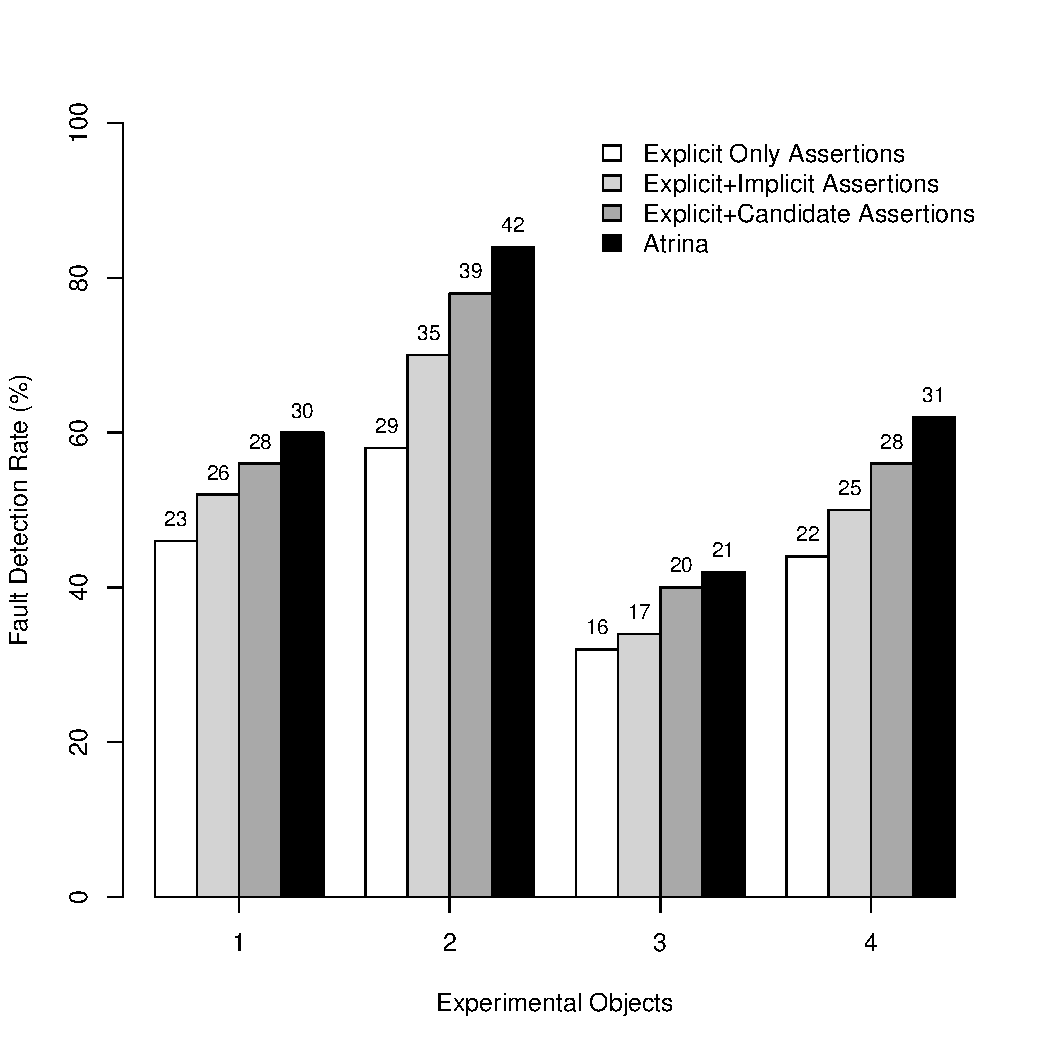
\includegraphics[width=1\hsize]{r-scripts/assertionTypeFaultDetec}
  \vspace{-0.18in} 
  \mycaption{Fault detection rate using different types of generated assertions.}
  \vspace{-0.1in} 
  \label{Fig:assertionTypeFaultDetec} 
\end{figure}
\headbf{Effectiveness (RQ2)} \figref{assertionTypeFaultDetec} depicts the fault detection rate achieved by (1) \tool, (2) explicit assertions when included individually, and (3) explicit assertions in conjunction with either implicit assertions or (4) candidate assertions. The number on each bar represent the number of faults detected by the corresponding assertion types. As shown in \figref{assertionTypeFaultDetec}, \tool detects on average 62\% of the total faults (ranges from 42-84\%).
The percentage of faults revealed by including only explicit assertions is always less than the ones that are detected through the combination of explicit with either implicit assertions or candidate assertions. This indicates that implicit as well as candidate assertions are essential entities in improving the fault finding capability of \tool. By eliminating implicit and candidate assertions, fault detection rate drops by 27\% on average and up to 31\% for the EnterpriseStore application (ID 2).

\figref{assertionTypeFaultDetec} shows that the improvement brought by implicit assertions is 8\% on average, however, when candidate assertions are included fault detection rate is increased by 21\% on average. This indicates that candidate assertions play a more prominent role in increasing the number of faults detected by \tool in comparison with implicit assertions. Not surprisingly, explicit assertions contribute the most among the other assertion types generated by \tool. Explicit assertions detect 73\% of the total faults on average (ranges from 69-77\%). These assertions are derived directly from the DOM-based oracles written by the developer of the application who has a deep knowledge of the application's behaviour. Therefore, it is expected that code-level assertions derived directly from such oracles have the highest impact on fault finding capability of our tool.        
\headbf{Comparison with human-written DOM-based Assertions (RQ3)}
\begin{figure}[!t]
  \centering
  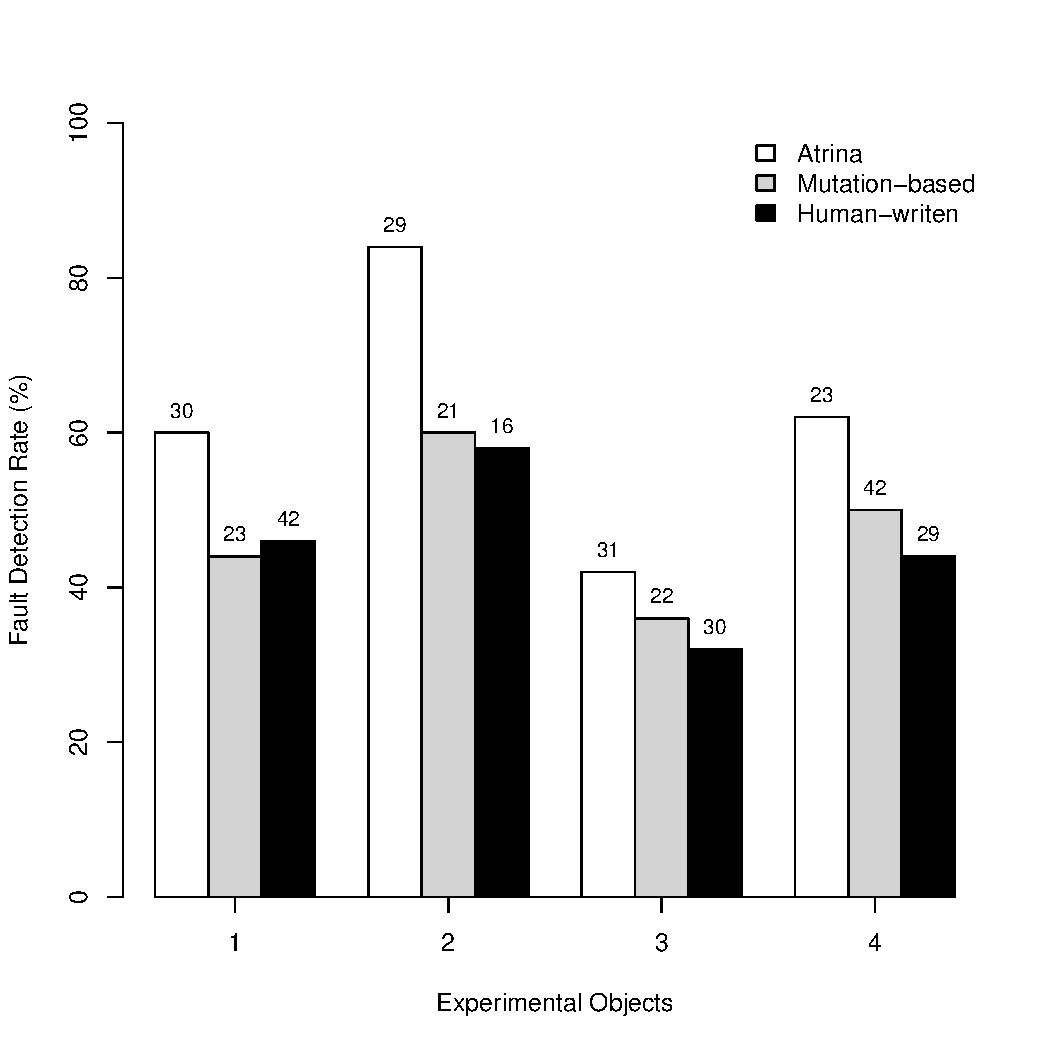
\includegraphics[width=1\hsize]{r-scripts/barplot-faultDetectionRate}
  \vspace{-0.18in}   
  \mycaption{Fault finding capability.}
  \vspace{-0.1in} 
  \label{Fig:barplot-faultDetectionRate}
\end{figure}
\figref{barplot-faultDetectionRate} depicts the fault detection rate achieved by the code-level assertions generated by \tool in comparison with the human-written DOM-based assertions. The numbers shown on each bar represent the number of faults detected by the corresponding assertion generation technique. As shown in the figure, the percentage of faults found by \tool is always higher than manually written DOM-based assertions. Overall, our approach outperforms manual assertions in terms of fault finding capability by 37\% on average (ranges from 30-45\%). We observed that on average 52\% of the candidate DOM properties that we select to construct our candidate assertions were ignored to check in human-written DOM assertions, although their value are updated through the \javascript code.
We further noticed that for each failed manual DOM assertion as a result of an injected fault, at least one explicit assertion fails in \tool (three failed explicit assertion on average). This indicates that exploiting the available knowledge of the tester in the written DOM oracles can help to produce fruitful set of code-level assertions. Moreover, in the experimental objects we observed that most often DOM assertions written by the tester are too generic in nature. Therefore even when a DOM assertion detects a \javascript fault, pinpointing the root cause of the error can be quite challenging. However, code-level assertions make it easier for the tester to localize the fault.

We observed in several cases that the value of a DOM element property which is checked in the human-written test suite is later used in a \javascript code that involves with internal computations only. If the seeded fault falls in the corresponding computational statements, the resulting error is not captured through the manually written DOM assertions. In such cases, implicit assertions are capable of detecting the error, which points to the importance of incorporating these types of assertions in our approach. We also noticed that around 33\% of the faults that are found by implicit assertions, while remain undetected by the human-written ones, requires executing a more complex sequence of events to propagate to the observable DOM (e.g., when an object's property is assigned in a function to be later used in updating a value of a DOM element after a specific event is triggered).    
\headbf{Comparison with Mutation-based Assertion Generation (RQ4)}
\figref{barplot-faultDetectionRate} presents the results of comparing fault finding capability of \tool with mutation-based assertion generation technique. As shown in the figure our approach produces unit assertions that are more effective than those produced by mutation-based technique. \tool surpasses mutation-based approach by 29\% on average (ranges from 17-40\%), despite the implementation and evaluation of mutation-based technique both use common mutation operators which favours towards mutation-based assertion generation as we discussed in \secref{setup}. This points to the importance of incorporating the valuable information exists in human-written DOM-based test suites.

While the results demonstrate that \tool is relatively more effective than mutation-based approach in terms of fault detection, we further investigate efficiency of our approach in terms of time overhead. We compute overhead of \tool as the summation of time required for (1) instrumenting the application and (2) analyzing the collected trace to compute \javascript slices. To calculate time overhead of the mutation-based approach, we consider the total time required for running the test suite multiple times (once per mutation), generating mutants, as well as the time needed to compare the original and the mutated version of the application to generate assertions.    
Our results show that the time overhead for \tool is 52 seconds on average, while the overhead computed for mutation-based technique is 123 seconds on average. This indicates that \tool significantly outperforms mutation-based assertion generation as far as time efficiency is concerned. Moreover, this points to the known performance shortcomings of approaches that rely on mutant generation.       


